%%%%%%%%%%%%%%%%%%%%%%%%%%%%%%%%%%%%%%%%%%%%%%%%%%%%%%%%%%%%%%%%%%%%%%%%%%%%%%%%%%%%%
%%%%%%%%%%%%%%%%%%%%%%%%%%%%%%%%%%%%%%%%%%%%%%%%%%%%%%%%%%%%%%%%%%%%%%%%%%%%%%%%%%%%%

\setbeamercolor{block title}{bg=white, fg=black}
\setbeamercolor{body}{bg=blue!20}

%%%%%%%%%%%%%%%%%%%%%%%%%%%%%%%%%%%%%%%%%%%%%%%%%%%%%%%%%%%%%%%%%%%%%%%%%%%%%%%%%%%%%
%%%%%%%%%%%%%%%%%%%%%%%%%%%%%%%%%%%%%%%%%%%%%%%%%%%%%%%%%%%%%%%%%%%%%%%%%%%%%%%%%%%%%

\begin{frame}
	\frametitle{Этапы исправления ошибки в программном коде}
	\begin{itemize}
		\item Воспроизведение
		\item \textbf{Локализация}
		\item Изучение
		\item Исправление
		\item Тестирование
	\end{itemize}
\end{frame}

%%%%%%%%%%%%%%%%%%%%%%%%%%%%%%%%%%%%%%%%%%%%%%%%%%%%%%%%%%%%%%%%%%%%%%%%%%%%%%%%%%%%%
%%%%%%%%%%%%%%%%%%%%%%%%%%%%%%%%%%%%%%%%%%%%%%%%%%%%%%%%%%%%%%%%%%%%%%%%%%%%%%%%%%%%%


\begin{frame}[fragile]
	\frametitle{Пример}
	GCC ломается на следующем файле:
	\begin{lstlisting}[style =crs_cpp]
extern int printf (const char *, ...);
static char
(safe_unary_minus_func_int8_t_s)(char si )
{
  return
    (si==(-128)) ?
    ((si)) : -si;
  ...
  2683 lines of code
\end{lstlisting}
\end{frame}


%%%%%%%%%%%%%%%%%%%%%%%%%%%%%%%%%%%%%%%%%%%%%%%%%%%%%%%%%%%%%%%%%%%%%%%%%%%%%%%%%%%%%
%%%%%%%%%%%%%%%%%%%%%%%%%%%%%%%%%%%%%%%%%%%%%%%%%%%%%%%%%%%%%%%%%%%%%%%%%%%%%%%%%%%%%

\begin{frame}
	\frametitle{Классический дельта-дебаггинг}
	Дано: $test$ и $c_x$, такие что $test(c_x) = fail$ \\
	Необходимо найти $c'_x = ddmin(c_x)$, такое что $c'_x \subseteq c_x, test(c'_x) = fail$ \\ \  \\ 
	$ddmin(c_x) = ddmin_2(c_x, 2)$ где \\
\[ ddmin_2(c'_x, n) =
  \begin{cases}
    ddmin_2(\Delta_i, 2)       & \quad \text{if } test(\Delta_i) = fail\\
    ddmin_2(\nabla_i, max(n - 1, 2))       & \quad \text{if } test(\nabla_i) = fail\\
    ddmin_2(c'_x, min(|c'_x|, 2n))       & \quad \text{if } n < |c'_x|\\
    c'_x
  \end{cases}
\]
\\
где $\nabla_i = c'_x - \Delta_i, c'_x = \Delta_1 \cup \Delta_2 \cup ... \cup \Delta_n$, все $\Delta_i$ попарно не пересекаются
\end{frame}

%%%%%%%%%%%%%%%%%%%%%%%%%%%%%%%%%%%%%%%%%%%%%%%%%%%%%%%%%%%%%%%%%%%%%%%%%%%%%%%%%%%%%
%%%%%%%%%%%%%%%%%%%%%%%%%%%%%%%%%%%%%%%%%%%%%%%%%%%%%%%%%%%%%%%%%%%%%%%%%%%%%%%%%%%%%
\definecolor{forest}{rgb}{0,0.7,0}

\begin{frame}[fragile]
	\frametitle{Пример}
\begin{minipage}[t]{0.48\linewidth}
		\begin{itemize}
		\item[] \{1, 2, 3, 4, 5, 6, 6, 8\} 
		\item[] \{1, 2, 3, 4\}			  
		\item[] \{5, 6, 6, 8\}
		\item[] \{5, 6\}
		\item[] \{6, 8\}
		\item[] \{5\}, \{6\}, \{6\}, \{8\}
		\item[] \{5, 6, 6\}
		\item[] \{5, 6\}
		\item[] \{6, 6\}
		\item[] \{6\}
		\item[] \{6\}
		\item[] \textbf{\{6, 6\}}
	\end{itemize}
\end{minipage}
\begin{minipage}[t]{0.48\linewidth}
		\begin{itemize}
		\item[] {\color{red}X}
		\item[] {\color{forest}V}	  
		\item[] {\color{red}X}
		\item[] {\color{forest}V}
		\item[] {\color{forest}V}
		\item[] {\color{forest}V}
		\item[] {\color{red}X}
		\item[] {\color{forest}V}
		\item[] {\color{red}X}
		\item[] {\color{forest}V}
		\item[] {\color{forest}V}
		\item[] {\color{red}X}
	\end{itemize}
\end{minipage}

\end{frame}

%%%%%%%%%%%%%%%%%%%%%%%%%%%%%%%%%%%%%%%%%%%%%%%%%%%%%%%%%%%%%%%%%%%%%%%%%%%%%%%%%%%%%
%%%%%%%%%%%%%%%%%%%%%%%%%%%%%%%%%%%%%%%%%%%%%%%%%%%%%%%%%%%%%%%%%%%%%%%%%%%%%%%%%%%%%

\begin{frame}[fragile]
	\frametitle{``Простой'' дельта-дебаггинг}
	\begin{itemize}
		\item Работает на уровне строк
		\item Не учитывает структуру кода
	\end{itemize}
	\begin{lstlisting}[style=crs_cpp]
void f() {
    int x;
    int y;
    if (x != 0) {
        y = x;
    } else {
        return 0;
    }
    while (y != 0) {
        y--;
    }
    return y;
}
\end{lstlisting}
\end{frame}

%%%%%%%%%%%%%%%%%%%%%%%%%%%%%%%%%%%%%%%%%%%%%%%%%%%%%%%%%%%%%%%%%%%%%%%%%%%%%%%%%%%%%
%%%%%%%%%%%%%%%%%%%%%%%%%%%%%%%%%%%%%%%%%%%%%%%%%%%%%%%%%%%%%%%%%%%%%%%%%%%%%%%%%%%%%
\lstset{escapeinside={<@}{@>}}
\begin{frame}[fragile]
	\frametitle{Дельта-дебаггинг + topformflat}
	\begin{minipage}{0.4\linewidth}
		\begin{lstlisting}[style=crs_cpp]
//Level = 1
void f() {
     int x;
     int y;
     if (x != 0) { x *= 3; y = x;}
     else {return 0;}
     while (y != 0) {y--;}
     return y;
 }
 \end{lstlisting}
	\end{minipage}
	\begin{minipage}{0.1\linewidth}
	\ \ 
	\end{minipage}
	\begin{minipage}{0.4\linewidth}
		\begin{lstlisting}[style=crs_cpp]
//Level = 1
fun f(): Int {
    var x = 1
    var y = 0
    if (x != 0) <@\textcolor{red}{\{ x *= 3 y = x \}}@>
    else { return 0 }
    while (y != 0) { --y }
    return y
}
 \end{lstlisting}
	\end{minipage}
	\\ \
	\center{ 
	Не подходит для языков, где переносы строки являются критичными}
\end{frame}

%%%%%%%%%%%%%%%%%%%%%%%%%%%%%%%%%%%%%%%%%%%%%%%%%%%%%%%%%%%%%%%%%%%%%%%%%%%%%%%%%%%%%
%%%%%%%%%%%%%%%%%%%%%%%%%%%%%%%%%%%%%%%%%%%%%%%%%%%%%%%%%%%%%%%%%%%%%%%%%%%%%%%%%%%%%

\begin{frame}
	\frametitle{Иерархический-дельта дебаггинг}
	\begin{figure}
		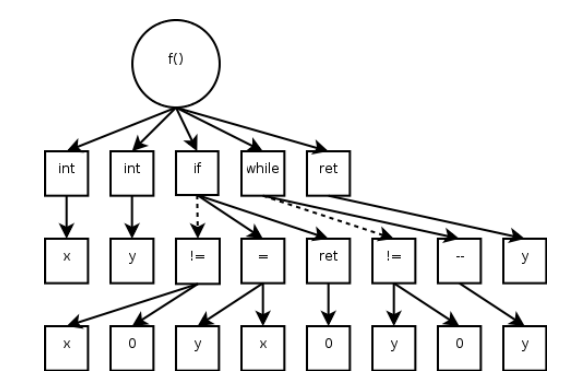
\includegraphics[width=100mm]{image/hddexample}
	\end{figure}	
\end{frame}

%%%%%%%%%%%%%%%%%%%%%%%%%%%%%%%%%%%%%%%%%%%%%%%%%%%%%%%%%%%%%%%%%%%%%%%%%%%%%%%%%%%%%
%%%%%%%%%%%%%%%%%%%%%%%%%%%%%%%%%%%%%%%%%%%%%%%%%%%%%%%%%%%%%%%%%%%%%%%%%%%%%%%%%%%%%

\begin{frame}
	\frametitle{Иерархический дельта-дебаггинг}
	\begin{algorithmic}
		\State $level \gets 0$
		\State $node \gets getNodesOfLevel(tree, 0)$
		\State while$(nodes \neq \emptyset)$ do
		\State \ \ \ \ $minconfig \gets DDMIN(nodes)$
		\State \ \ \ \ $delete(tree, level, minconfig)$
		\State \ \ \ \ $level \gets level + 1$
		\State \ \ \ \ $nodes \gets getNodesOfLevel(tree, level)$
		\State $end while$
		
	\end{algorithmic}
\end{frame}


%%%%%%%%%%%%%%%%%%%%%%%%%%%%%%%%%%%%%%%%%%%%%%%%%%%%%%%%%%%%%%%%%%%%%%%%%%%%%%%%%%%%%
%%%%%%%%%%%%%%%%%%%%%%%%%%%%%%%%%%%%%%%%%%%%%%%%%%%%%%%%%%%%%%%%%%%%%%%%%%%%%%%%%%%%%

\begin{frame}
	\frametitle{Иерархический дельта-дебаггинг}
	\begin{figure}
		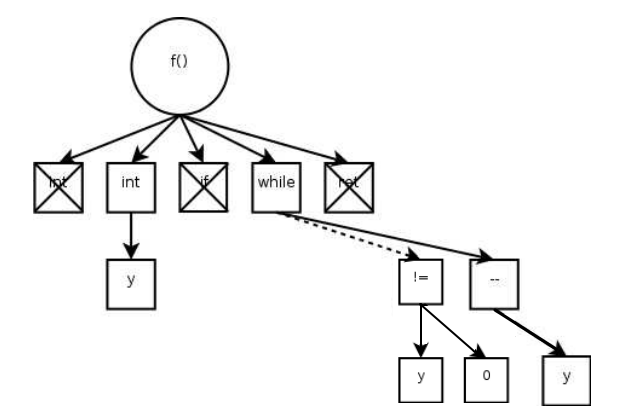
\includegraphics[width=100mm]{image/hdd}
	\end{figure}	
\end{frame}

%%%%%%%%%%%%%%%%%%%%%%%%%%%%%%%%%%%%%%%%%%%%%%%%%%%%%%%%%%%%%%%%%%%%%%%%%%%%%%%%%%%%%
%%%%%%%%%%%%%%%%%%%%%%%%%%%%%%%%%%%%%%%%%%%%%%%%%%%%%%%%%%%%%%%%%%%%%%%%%%%%%%%%%%%%%

\begin{frame}
	\frametitle{Существующие инструменты}
	\begin{itemize}
		\item Picireny
			\begin{itemize}
				\item Иерархический дельта-дебаггер
				\item ANTLR v4 grammar
				\item Rule
			\end{itemize}
		\item Creduce (Delta)
			\begin{itemize}
				\item Редуктор для языка C
				\item Состоит из набора трансформаций над исходным кодом
				\item 57 компиляторных багов
				\begin{itemize}
					\item Delta: 8600 байт
					\item Creduce: 120 байт
				\end{itemize}
			\end{itemize}
	\end{itemize}
\end{frame}
%%%%%%%%%%%%%%%%%%%%%%%%%%%%%%%%%%%%%%%%%%%%%%%%%%%%%%%%%%%%%%%%%%%%%%%%%%%%%%%%%%%%%
%%%%%%%%%%%%%%%%%%%%%%%%%%%%%%%%%%%%%%%%%%%%%%%%%%%%%%%%%%%%%%%%%%%%%%%%%%%%%%%%%%%%%

\begin{frame}
	\frametitle{Мотивация}
	\begin{itemize}
		\item Существует генератор случайных тестов для компилятора котлина
		\item Зачастую компиляторные баги находятся в очень больших проектах
	\end{itemize}
\end{frame}
%%%%%%%%%%%%%%%%%%%%%%%%%%%%%%%%%%%%%%%%%%%%%%%%%%%%%%%%%%%%%%%%%%%%%%%%%%%%%%%%%%%%%
%%%%%%%%%%%%%%%%%%%%%%%%%%%%%%%%%%%%%%%%%%%%%%%%%%%%%%%%%%%%%%%%%%%%%%%%%%%%%%%%%%%%%

\begin{frame}
	\frametitle{ReduKtor}
	\begin{itemize}
		\item Специфичные для Котлина peephole трансформации
			\begin{itemize}
				\item x += y -> x = y
				\item val s: String = t ?: '''' -> val s: String = ''''
				\item while -> if
				\item ...
			\end{itemize}
		\item Иерархический дельта-дебаггинг
		\item Слайсинг
		\item Трансформации над PSI
			\begin{itemize}
				\item Упрощение when
				\item Замена тела функции на константу
				\item Инлайнинг
				\item Переименование переменных
				\item ...
			\end{itemize}
	\end{itemize}
\end{frame}

%%%%%%%%%%%%%%%%%%%%%%%%%%%%%%%%%%%%%%%%%%%%%%%%%%%%%%%%%%%%%%%%%%%%%%%%%%%%%%%%%%%%%
%%%%%%%%%%%%%%%%%%%%%%%%%%%%%%%%%%%%%%%%%%%%%%%%%%%%%%%%%%%%%%%%%%%%%%%%%%%%%%%%%%%%%

\begin{frame}
	\frametitle{Прогресс}
	На данный момент реализованы:
	\begin{itemize}
		\item Некоторые peephole трансформации
		\item Алгоритм иерархического дельта-дебаггинга
		\item Система для запуска трансформаций и проверки результирующих программ
		\item Работает для компиляторных тестов и обычных программ (необходимые свойства поведения программы задаются с помощью скрипта)
	\end{itemize}
\end{frame}

%%%%%%%%%%%%%%%%%%%%%%%%%%%%%%%%%%%%%%%%%%%%%%%%%%%%%%%%%%%%%%%%%%%%%%%%%%%%%%%%%%%%%
%%%%%%%%%%%%%%%%%%%%%%%%%%%%%%%%%%%%%%%%%%%%%%%%%%%%%%%%%%%%%%%%%%%%%%%%%%%%%%%%%%%%%

\begin{frame}
	\frametitle{Планы на будущее}
	\begin{itemize}
		\item Больше трансформаций
		\item Редукция проектов целиком
		\item Поддержка языка Java
		\item Апробация на реальных багах
	\end{itemize}
\end{frame}

%%%%%%%%%%%%%%%%%%%%%%%%%%%%%%%%%%%%%%%%%%%%%%%%%%%%%%%%%%%%%%%%%%%%%%%%%%%%%%%%%%%%%
%%%%%%%%%%%%%%%%%%%%%%%%%%%%%%%%%%%%%%%%%%%%%%%%%%%%%%%%%%%%%%%%%%%%%%%%%%%%%%%%%%%%%

\begin{frame}[fragile]
\frametitle{Контакты}
\texttt{stepanov@kspt.icc.spbstu.ru} \\ \ \\ \ \\
ReduKtor repository: \texttt{https://bitbucket.org/vorpal-research/reduktor}
\\ \ \\ 
\begin{columns} 
\column{0.33\textwidth} 
	\begin{figure}
		
\includegraphics[width=0.99\linewidth]{image/polytech_logo_en} 
	\end{figure}
\column{0.33\textwidth} 
	\begin{figure}
		
\includegraphics[width=0.99\linewidth]{image/jetbrainsLogo} 
	\end{figure}
\end{columns}
\end{frame}
